\documentclass[12pt]{article}

\nofiles  % TeX does not produce an *.aux file
\usepackage{color}
\usepackage{graphicx}
\usepackage{fix-cm}
\input{/Users/nychka/Home/Tex/NychkaStuff.tex}
 \input{/Users/nychka/Home/Tex/ColorsFromR.tex}
\renewcommand{\baselinestretch}{1.1}
\setlength{\paperheight}{11in}
\setlength{\paperwidth}{8.5in}
\setlength{\textheight}{8.75in}
\setlength{\textwidth}{6.75in}
\setlength{\evensidemargin}{0.0in}
\setlength{\oddsidemargin}{0.0in}
\setlength{\topmargin}{0in}
\setlength{\parindent}{0in}
\setlength{\parskip}{12pt}
\pagestyle{empty}

  
\begin{document}
\vspace*{-1.5in}
{\sf
{ 
\color{grey40}
\hspace*{-.5in} \fontsize{35}{50}\selectfont{ 
Introduction to Data Analysis  
with R 
}
}
\\

%\hspace*{-.25in}
\begin{minipage}{7in}{\Large 
APPM 2720:  3 - 4:15 PM, Monday/Wednesday,  Spring 2017  \\ \\
 Douglas Nychka, 
Affiliate Faculty, Applied Mathematics  \\
Senoir Scientist, National Center for Atmospheric Research \\
\verb+nychka@ucar.edu+
%Scientific Staff, National Center for Atmospheric Research
 }
 \end{minipage}
\\

\begin{minipage}{6.75in}
{\Large 
{\it Data science}  is a new field that combines mathematics, computer science, and statistics with the goal of
answering questions and gaining new insights from data. 
}
\end{minipage}

%\hspace{-.25in}

%\end{quote}
%\hspace{-.25in}

\begin{minipage}{4in}
\vspace*{0in}
{
%\begin{itemize}
\bdot How should I buy  a used car on {\tt cars.com}? \\[.125in]
\bdot Where is the steepest part of a ski slope? \\[.125in] 
\bdot How is the climate changing in Colorado? \\[.125in] 
\bdot When will the next flu outbreak occur? \\[.125in] 
\bdot How do you build a spam filter for email?
%\end{itemize}
}
%
\end{minipage}
%
\begin{minipage}{3.75in}
\vspace*{0in}
\hspace*{.375in} Asking prices for Audi A4s \\
\hspace*{.125in}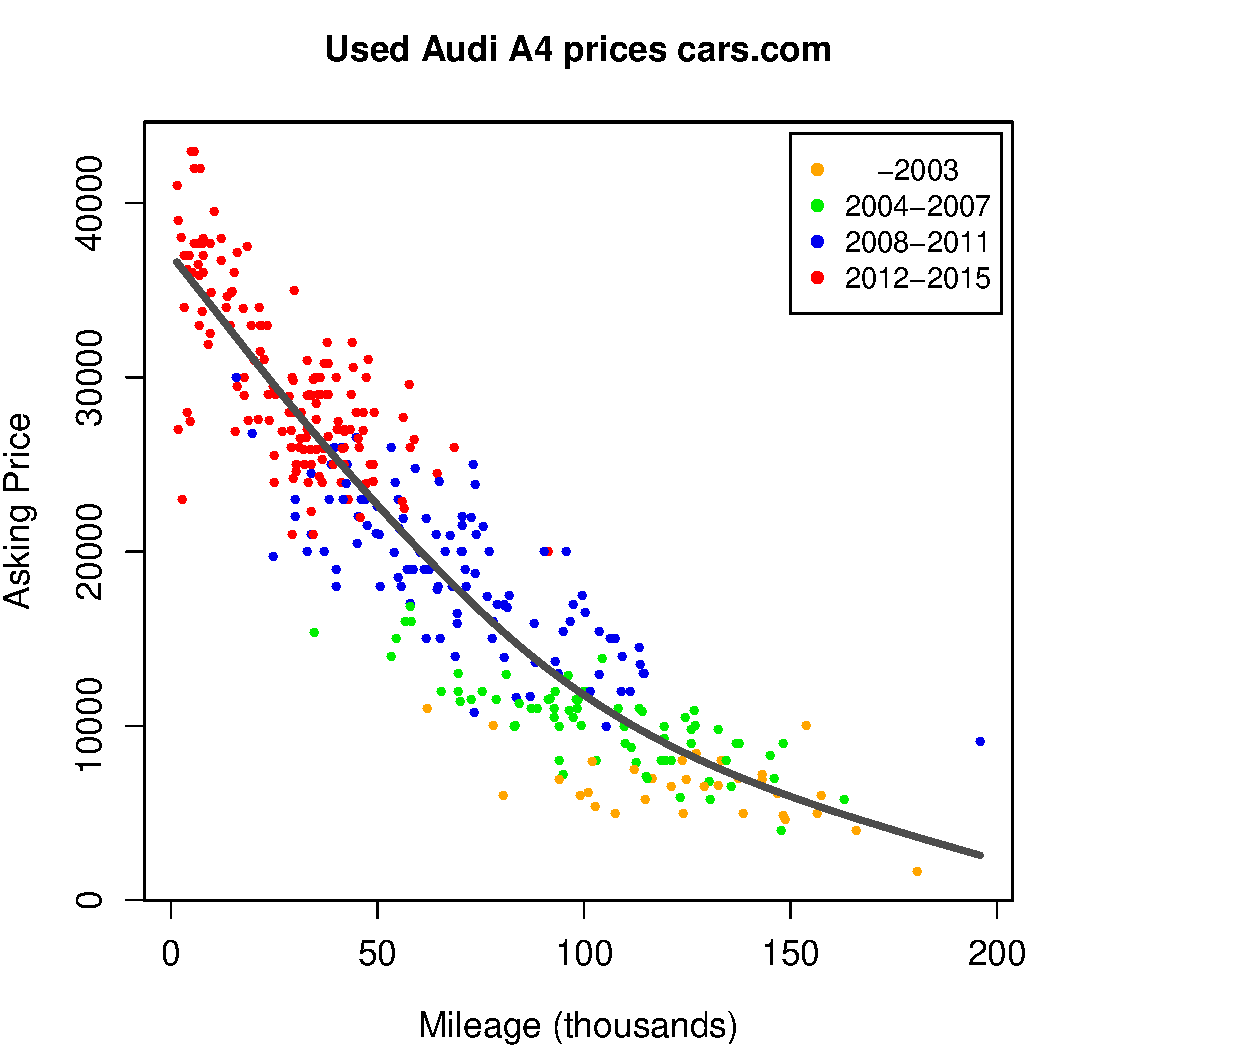
\includegraphics[width=2.25in]{A4.pdf}
\end{minipage}
\\

\begin{minipage}[t]{3.75in}
\vspace*{0in}
\hspace*{.25in} 
Daily precipitation amounts  for Boulder \\
%\hspace*{.25in}\includegraphics[width=3.5in, height=3in]{/Users/nychka/Home/Current_talks/AGUExtremes/pix/Boulder1.pdf} 
%\hspace*{.25in}
\includegraphics[width=3.25in, height=2in]{Boulder1.pdf} 
\end{minipage}
%\hspace*{-.25in}
\begin{minipage}[t]{3.75in}
\vspace*{0in}
Degree of slope for Riflesight Notch Ski Trail \\
Mary Jane, Colorado  \\
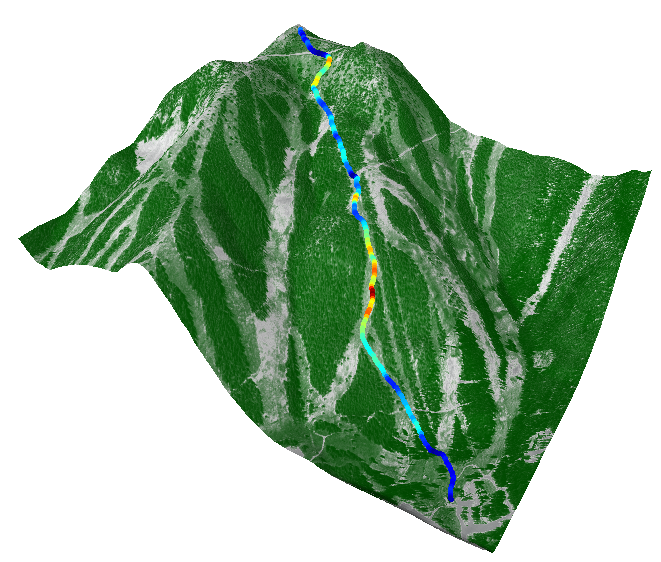
\includegraphics[width=2.75in]{slopeimage3.png}
\end{minipage}
%
{
This course will expose students to practical data analysis and statistics. In the process students will learn how to 
 write programs in the R language, interpret their results,  generate figures and reports, and handle large data sets. 
 The course will also introduce students to  modern data analysis tools including 
regression and smoothing, multivariate analysis, clustering,  and image analysis. Grading will be based on weekly homework, 
several take home quizes and a focused data analysis project.  Check out last years course at: \verb+https://github.com/NCAR/DataAnalysis101+ 
}
}
\end{document}
